% \documentclass[a4paper, 11pt]{article}
\documentclass{article}

\usepackage[dvipsnames]{xcolor}
\usepackage{ctex}
\usepackage{graphicx}
\usepackage[unicode]{hyperref}
\usepackage{cite}
\usepackage{indentfirst}
\usepackage{listings}
\usepackage{geometry}
\usepackage{amsmath}
\usepackage{tabularx}

\geometry{a4paper, left=2cm, right=2cm, top=1cm, bottom=1.5cm}

% \lstset{
%   language=C++,
%   basicstyle=\fontsize{8}{5}\ttfamily, % 设置代码字体大小为 12pt
%   breaklines=true, % 自动换行
%   numbers=left,
%   showstringspaces = false
% }

%%%%%% 设置字号 %%%%%% 
\newcommand{\chuhao}{\fontsize{nn42pt}{\baselineskip}\selectfont}
\newcommand{\xiaochuhao}{\fontsize{36pt}{\baselineskip}\selectfont}
\newcommand{\yihao}{\fontsize{28pt}{\baselineskip}\selectfont}
\newcommand{\erhao}{\fontsize{21pt}{\baselineskip}\selectfont}
\newcommand{\xiaoerhao}{\fontsize{18pt}{\baselineskip}\selectfont}
\newcommand{\sanhao}{\fontsize{15.75pt}{\baselineskip}\selectfont}
\newcommand{\sihao}{\fontsize{14pt}{\baselineskip}\selectfont}
\newcommand{\xiaosihao}{\fontsize{12pt}{\baselineskip}\selectfont}
\newcommand{\wuhao}{\fontsize{10.5pt}{\baselineskip}\selectfont}
\newcommand{\xiaowuhao}{\fontsize{9pt}{\baselineskip}\selectfont}
\newcommand{\liuhao}{\fontsize{7.875pt}{\baselineskip}\selectfont}
\newcommand{\qihao}{\fontsize{5.25pt}{\baselineskip}\selectfont}

% %%%% 设置 section 属性 %%%%
% \makeatletter
% \renewcommand\section{\@startsection{section}{1}{\z@}%
% {-1.5ex \@plus -.5ex \@minus -.2ex}%
% {.5ex \@plus .1ex}%
% {\normalfont\sihao\CJKfamily{hei}}}
% \makeatother

 %%%% 设置 subsection 属性 %%%%
% \makeatletter
% \renewcommand\subsection{\@startsection{subsection}{1}{\z@}%
% % {-1.25ex \@plus -.5ex \@minus -.2ex}%
% % {-1ex \@plus -.5ex \@minus -.2ex}%
% {-1ex \@plus -.3ex \@minus -.1ex}%
% {.4ex \@plus .1ex}%
% {\normalfont\xiaosihao\CJKfamily{hei}}}
% \makeatother

% %%%% 设置 subsubsection 属性 %%%%
% \makeatletter
% \renewcommand\subsubsection{\@startsection{subsubsection}{1}{\z@}%
% {-1ex \@plus -.5ex \@minus -.2ex}%
% {.3ex \@plus .1ex}%
% {\normalfont\xiaosihao\CJKfamily{hei}}}
% \makeatother

%%%% 段落首行缩进两个字 %%%%
\makeatletter
\let\@afterindentfalse\@afterindenttrue
\@afterindenttrue
\makeatother
% \setlength{\parindent}{2em}  %中文缩进两个汉字位

%%%% 下面的命令重定义页面边距,使其符合中文刊物习惯 %%%%
% \addtolength{\topmargin}{-54pt}
% \setlength{\oddsidemargin}{0.63cm}  % 3.17cm - 1 inch
% \setlength{\evensidemargin}{\oddsidemargin}
% \setlength{\textwidth}{14.66cm}
% \setlength{\textheight}{24.00cm}    % 24.62

%%%% 下面的命令设置行间距与段落间距 %%%%
\linespread{1.0}
% \setlength{\parskip}{1ex}
\setlength{\parskip}{0.5\baselineskip}

% 在导言区进行样式设置
\lstset{
    language=C++, % 设置语言
 	basicstyle=\ttfamily, % 设置字体族
 	breaklines=true, % 自动换行
 	keywordstyle=\bfseries\color{NavyBlue}, % 设置关键字为粗体,颜色为 NavyBlue
 	morekeywords={PressureSensor, Button, Oled}, % 设置更多的关键字,用逗号分隔
 	emph={self}, % 指定强调词,如果有多个,用逗号隔开
    emphstyle=\bfseries\color{Rhodamine}, % 强调词样式设置
    commentstyle=\itshape\color{black!50!white}, % 设置注释样式,斜体,浅灰色
    stringstyle=\bfseries\color{PineGreen!90!black}, % 设置字符串样式
    columns=flexible,
    numbers=left, % 显示行号在左边
    numbersep=2em, % 设置行号的具体位置
    numberstyle=\footnotesize, % 缩小行号
    % frame=single, % 边框
	tabsize = 4,  %行缩进
    framesep=1em % 设置代码与边框的距离
}

%%%% 正文开始 %%%%
\begin{document}	
		%%%% 定理类环境的定义 %%%%
\newtheorem{example}{例}             % 整体编号
\newtheorem{algorithm}{算法}
\newtheorem{theorem}{定理}[section]  % 按 section 编号
\newtheorem{definition}{定义}
\newtheorem{axiom}{公理}
\newtheorem{property}{性质}
\newtheorem{proposition}{命题}
\newtheorem{lemma}{引理}
\newtheorem{corollary}{推论}
\newtheorem{remark}{注解}
\newtheorem{condition}{条件}
\newtheorem{conclusion}{结论}
\newtheorem{assumption}{假设}

		%%%% 重定义 %%%%
\renewcommand{\contentsname}{目录}  % 将Contents改为目录
\renewcommand{\abstractname}{摘要}  % 将Abstract改为摘要
\renewcommand{\refname}{参考文献}   % 将References改为参考文献
\renewcommand{\indexname}{索引}
\renewcommand{\figurename}{图}
\renewcommand{\tablename}{表}
\renewcommand{\appendixname}{附录}
\renewcommand{\algorithm}{算法}	

		%%% 定义标题格式,包括title,author,affiliation,email等 %%%%
\title{智能仓储系统的开发研究}
% \author{XXX\footnote{电子邮件: XXXXXXXXXXXX@zjut.edu.cn 学号: XXXXXXXXXXXX}\\[2ex]
% \xiaosihao 浙江工业大学\\[2ex]}
\author{\xiaosihao 先进计算与机器人研究所}
%\date{}
		
		%%%% 以下部分是正文 %%%%  
\maketitle
		
\tableofcontents
\newpage

\section{第四章: I2C通信}
\begin{figure}[h]
    \centering
    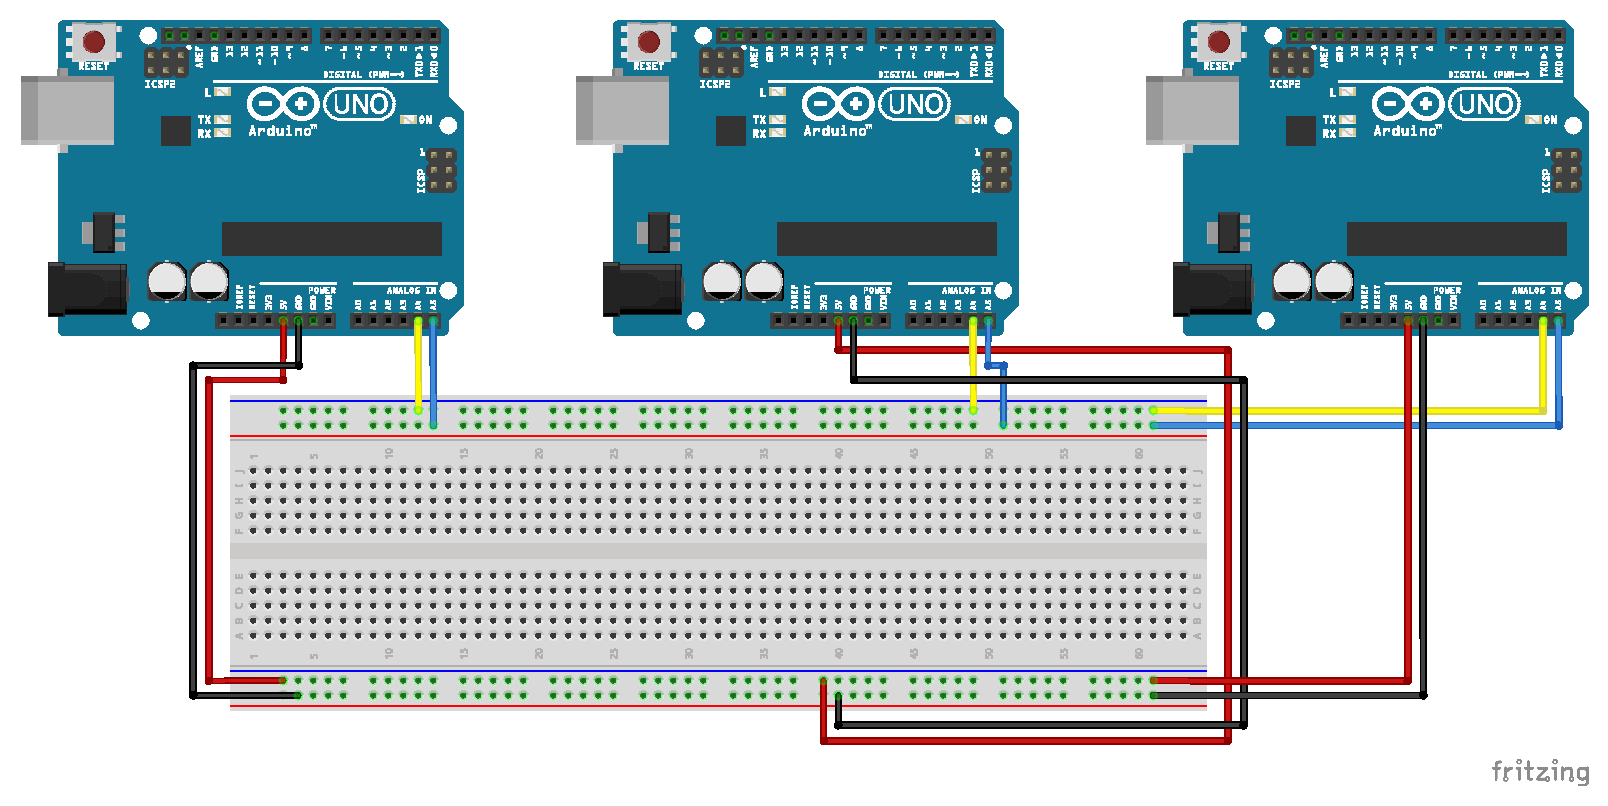
\includegraphics[width=0.6\linewidth]{../picture/I2C_.pdf}
    \caption{Wire板间通信电路图}
    \label{fig:Wire板间通信电路图}
\end{figure}

\begin{figure}[h]
     \centering
     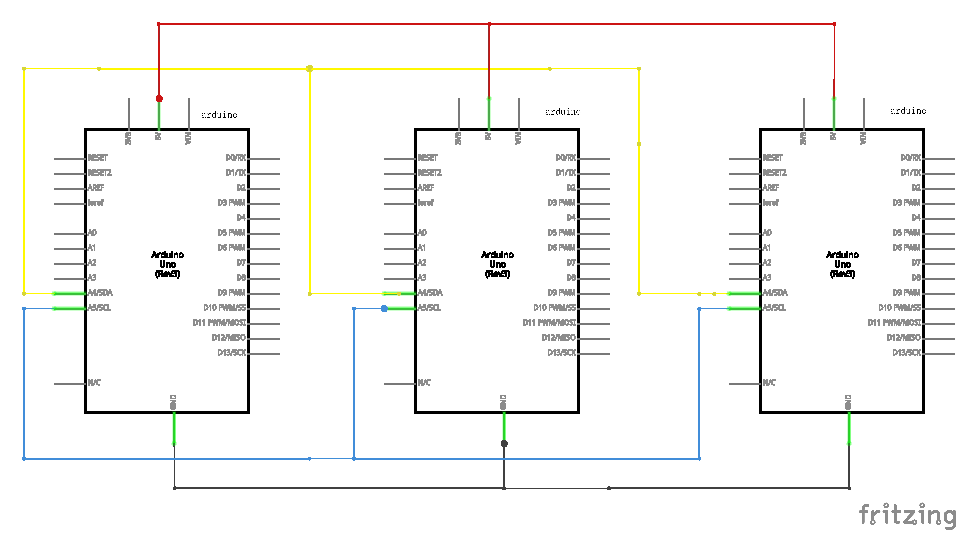
\includegraphics[width=0.6\linewidth]{../picture/I2C_line.pdf}
     \caption{Wire板间通讯电路原理图}
     \label{fig:Wire板间通讯电路原理图}
\end{figure}

\begin{itemize}
  \item IIC通信开始之前需要确定主从机地址。主机用Master类表示, 从机用Slave类表示, 主从机可以互相按地址发送消息。
  \item Message类中会规定发送的消息格式, 以及消息发送前的打包和消息收到后的解包。
\end{itemize} 

\subsection{Master}
Master类的核心变量是发送的字符数组Data, 主机的地址address。为了便于Slave类继承, 就设成公共变量。
\begin{lstlisting}
#include <Wire.h>
#include <Arduino.h>
#include <string.h>

class Master {
public:
  int address;
  char Data[17];
static bool Gotitflag;

  Master(int add);
  void init();
  void Set_Data(String message);
  void Send(int slave_add);
  bool isData_receivedNull();
static void receiveEvent(int howmany);
};
\end{lstlisting}

在构造函数Master中, 通过赋值更新地址address。
\begin{lstlisting}
Master::Master(int add){
  address=add;
};
\end{lstlisting}

由于Wire.begin()不能在setup之前运行, 所以在初始化函数init中初始化了IIC通信, 并绑定了回调函数receiveEvent, 在IIC收到消息时调用。
\begin{lstlisting}
void Master::init() {
  Wire.begin(address);
  Wire.onReceive(receiveEvent);
  memset(Data, '0', 16);
};  
\end{lstlisting}

Set\_Data通过赋值更新Data。
\begin{lstlisting}
void Master::Set_Data(String message) {
  for (int i=0; i<message.length(); i++)
    Data[i] = message[i];
};  
\end{lstlisting}

Send是主机向地址为slave\_add的从机发送消息Data, 为了方便判断是否发送了, 发送成功则会在串口打印"Sended", 否则就会卡住, 不打印"Sended"。 
\begin{lstlisting}
void Master::Send(int slave_add) {
  Wire.beginTransmission(slave_add);
  Wire.write(Data);
  Wire.endTransmission(slave_add);
  Serial.println("Sended");
};
\end{lstlisting}

为了确认从机是否收到完整消息, 在下一节从机Slave类中会提到, 当Slave确认收到了完整消息, 就会向主机发送一个字符串"Gotit!"。那么相应地, 
主机也需要判断接收到的是不是"Gotit!"。如果是则会将一个静态变量Gotitflag置为1, 在演示代码Master.ino中, 会再次提到Gotitflag。
\begin{lstlisting}
bool Master::Gotitflag = 0;

void Master::receiveEvent(int howmany){
  String standard = "Gotit!";
  String buffer = "";
  while (Wire.available()) 
    buffer += (char) Wire.read();
  Serial.println(buffer);
  for (int i=0; i<6; i++)
    if (buffer[i] == standard[i])
      Gotitflag = 1;
};  
\end{lstlisting}

\subsubsection{Master.ino}
演示代码实现的是地址为8的主机会一直向地址为11的从机发送字符串"SS0812345RR", 直到Gotitflag置为1。 
Gotitflag置为1意味着从机发送回了收到的信号。则在串口打印结束发送。
\begin{lstlisting}
#include "Master.h"

Master master(8);

void setup() {
  Serial.begin(9600);
  master.init();
  master.Set_Data("SS0812345RR");
}

void loop() {
  while (!master.Gotitflag) {
    master.Send(11);
    delay(5000);
  }
  Serial.println("endsending");
  delay(500);
}
  
\end{lstlisting}

\subsection{Slave}
Slave类的核心变量是储存主机发送过来的完整消息Data\_received, 储存主机的地址address\_to\_send。
Slave储存自身的地址变量是从Master类中继承过来的。
\begin{lstlisting}
#include "Master.h"

class Slave : public Master{
private:
static String Data_received;

public:
static int address_to_send;

  Slave(int add);
  void init();
  void feedback();
static void slave_receiveEvent(int howmany);
};  
\end{lstlisting}

构造函数Slave()完全继承于Master的构造函数
\begin{lstlisting}
Slave::Slave(int add) : Master(add) {};  
\end{lstlisting}

初始化需要重定义, 因为回调函数slave\_receiveEvent与Master类的receiveEvent不一样。
\begin{lstlisting}
void Slave::init(){
  Wire.begin(address);
  Wire.onReceive(slave_receiveEvent);
  memset(Data, '0', 16);
}  
\end{lstlisting}

从机的回调函数slave\_receiveEvent需要在有消息的时候判断, 是不是"SS"开头, 如果是, 则开始读, 并更新Data\_received。并在读到"RR"时, 结束
更新Data\_received。结束更新后, 需要读取指定位置表示主机地址的字符。这里退出while循环需要严格以Wire.available()为准, 如果是读到完整消息
就直接退出, 很可能出现附录中第一节消息堵塞之陷入死循环。
\begin{lstlisting}
void Slave::slave_receiveEvent(int howmany){
  memset(&Data_received, 0, Data_received.length());
  bool addressflag = 1;
  while(Wire.available()) {
    Serial.println("connect");
    if (Data_received[0] != 'S' && Data_received[1] != 'S') {
      char start1 = (char) Wire.read();
      if (start1 == 'S') {
        char start2 = (char) Wire.read();
        if (start2 == 'S') {
          Data_received += 'S';
          Data_received += 'S';
        } 
      }
    }

    if (Data_received[0] == 'S' && Data_received[1] == 'S') {
      if (Data_received[Data_received.length()-2]=='R' && Data_received[Data_received.length()-1]=='R') {
        Wire.read();
        if (addressflag) {
          String address;
          for (int i=0; i<2; i++) address += Data_received[2+i];
          address_to_send = address.toInt();
          addressflag = 0;
        }
      } else {
        char end1 = (char) Wire.read();
        Data_received += end1;
        // Serial.println(Data_received);
      }
    }
  }
  Serial.println(address_to_send);
};  
\end{lstlisting}

在上一节Master类中有提到"Gotit!"作为从机读到完整消息的反馈。这里address\_to\_send是先设为不可能有的地址99, 在slave\_receiveEvent中, 
如果接收到完整消息, 则address\_to\_send会更新为有效地址, 所以利用address\_to\_send作为要不要发送"Gotit!"的flag。
\begin{lstlisting}
void Slave::feedback() {
  if (address_to_send!=99) {
    Wire.beginTransmission(address_to_send);
    Wire.write("Gotit!");
    Wire.endTransmission(address_to_send);
    address_to_send = 99;
  }  
};  
\end{lstlisting}

\subsubsection{Slave.ino}
演示代码是实现slave接收到IIC通信传来得的消息后, 反馈"Gotit!"给发送过来的主机。
\begin{lstlisting}
#include "Slave.h"

Slave slave(11);

void setup() {
  Serial.begin(9600);
  slave.init();
}

void loop() {
  slave.feedback();
  delay(500);
}  
\end{lstlisting}

\subsection{Message}
Message类的核心变量有5个, 储存完整消息的字符数组Data, 物品种类Type, 发送方地址DeviceAddress, 物品种类Amount, 物品总质量TotalMass。
关于字符数组的长度设置原因详见本章附录。由于unsigned long方便转化成char*, 而char*不便于计算有效长度, 故需要在转化前就通过数值确定
转化后的长度, 储存在totalmass\_str\_len中。
\begin{lstlisting}
#include <Arduino.h>
#include <string.h>

class Message {
private:
  char Data[17];
  char Type[3];
  int DeviceAddress, Amount;
  unsigned long TotalMass;
  int totalmass_str_len;

public:
  Message();
  
  void Set_Messagevalues(char *type, int device, int amount, unsigned long totalmass);
  void pack();
  void Output_pack();

  void Set_Data(char* message);
  void unpack();
  void Output_unpack();
};
\end{lstlisting}

构造函数里会对五个核心变量储存完整消息的字符数组Data, 物品种类Type, 发送方地址DeviceAddress, 物品种类Amount, 物品总质量TotalMass进行赋值。
这里规定消息前两位和后两位是标志位。"SS"表示消息开头, "RR"表示消息结尾。
\begin{lstlisting}
Message::Message() {
  memset(Data, '0', 16);
  Data[0] = 'S';
  Data[1] = 'S';
  Data[14] = 'R';
  Data[15] = 'R';
  Type[0] = '0';
  Type[1] = '0';
  DeviceAddress = 0;
  Amount = 0;
  TotalMass = 0;
}
\end{lstlisting}

Set\_Messagevalues通过赋值更新物品种类Type, 发送方地址DeviceAddress, 物品种类Amount, 物品总质量TotalMass, 长度totalmass\_str\_len。
\begin{lstlisting}
void Message::Set_Messagevalues(char *type, int device, int amount, unsigned long totalmass) {
  Type[0] = type[0];  //物品种类
  Type[1] = type[1];

  DeviceAddress = device;
  Amount = amount;
  TotalMass = totalmass;
  if (totalmass<10) totalmass_str_len = 1;
  else if (totalmass<100) totalmass_str_len = 2;
  else if (totalmass<1000) totalmass_str_len = 3;
  else if (totalmass<10000) totalmass_str_len = 4;
};
\end{lstlisting}

pack用物品种类Type, 发送方地址DeviceAddress, 物品种类Amount, 物品总质量TotalMass更新Data。unsigned long不能用String强制转换,
但可以用sprintf转化成char*。
\begin{lstlisting}
void Message::pack() {
  String device_str = String(DeviceAddress);
  String amount_str = String(Amount);
  char totalmass_str[5];
  sprintf(totalmass_str, "%d", TotalMass);

  for (int i=0; i<2; i++) 
    Data[2+i] = Type[i];  //物品种类

  int device_str_len = device_str.length();
  if (device_str_len == 1) {         //发送方地址
    Data[5] = device_str[0];
  }
  else if (device_str_len == 2) {
    Data[4] = device_str[0];
    Data[5] = device_str[1];
  }

  int amount_str_len = amount_str.length();   //物品数量
  if (amount_str_len == 1) Data[9] = amount_str[0];
  else if (amount_str_len == 2) 
    for (int i=0; i<2; i++) Data[8+i] = amount_str[i];
  else if (amount_str_len == 3) 
    for (int i=0; i<3; i++) Data[7+i] = amount_str[i];
  else if (amount_str_len == 4) 
    for (int i=0; i<4; i++) Data[6+i] = amount_str[i];

  if (totalmass_str_len == 1)    //物品总质量
    Data[13] = totalmass_str[0];
  else if (totalmass_str_len == 2)
    for (int i=0; i<2; i++) Data[12+i] = totalmass_str[i];
  else if (totalmass_str_len == 3)
    for (int i=0; i<3; i++) Data[11+i] = totalmass_str[i];
  else if (totalmass_str_len == 4)
    for (int i=0; i<4; i++) Data[10+i] = totalmass_str[i];
};
\end{lstlisting}

Output\_pack将打包后的Data打印在串口。
\begin{lstlisting}
void Message::Output_pack() {
  Serial.print("Data:");
  Serial.println(Data);
};  
\end{lstlisting}

Set\_Data通过赋值更新Data。
\begin{lstlisting}
void Message::Set_Data(char* message) {
  for (int i=2; i<14; i++) 
    Data[i]=message[i];
}  
\end{lstlisting}

pack用Data更新物品种类Type, 发送方地址DeviceAddress, 物品种类Amount, 物品总质量TotalMass。中间用字符串device\_str, amount\_str, tm\_str过渡,
然后用toInt转化成数值。
\begin{lstlisting}
void Message::unpack() {
  String device_str, amount_str;
  char totalmass_str[5];
  
  for (int i=0; i<2; i++)
    Type[i] = Data[2+i];

  for (int i=0; i<2; i++)
    device_str += Data[4+i];
  DeviceAddress = device_str.toInt();

  for (int i=0; i<4; i++) 
    amount_str += Data[6+i];
  Amount = amount_str.toInt();

  String tm_str;
  for (int i=10; i<14; i++) 
    tm_str += Data[i];
  TotalMass = tm_str.toInt(); 
};
\end{lstlisting}

Output\_unpack将打包后的物品种类Type, 发送方地址DeviceAddress, 物品种类Amount, 物品总质量TotalMass打印在串口。
\begin{lstlisting}
void Message::Output_unpack() {
  Serial.print("Type:");
  Serial.println(Type);
  Serial.print("DeviceAddress:");
  Serial.println(DeviceAddress);
  Serial.print("Amount:");
  Serial.println(Amount);
  Serial.print("TotalMass:");
  Serial.println(TotalMass);
};  
\end{lstlisting}

\subsubsection{Message.ino}
演示代码1是实现消息发送前的打包:
\begin{lstlisting}
#include "Message.h"
    
Message message;
    
char type[2] = {'0', '3'};   //unpack
int address = 8;
int num = 321;
unsigned long totalmass=19;
    
void setup() {
  Serial.begin(9600);
  message.Set_Messagevalues(type, address, num, totalmass);      //pack
  message.pack();
}
    
void loop() {
  message.Output_pack(); //pack
  delay(500);
}  
\end{lstlisting}  

演示代码2是实现消息收到后的解包:
\begin{lstlisting}
#include "Message.h"
  
Message message;

char data[17] = {'S','S','0','4','0','9','0','5','0','5','2','0','0','0','R','R'};   //pack
  
void setup() {
  Serial.begin(9600);
  message.Set_Data(data);  //unpack
  message.unpack();
}
  
void loop() {
  message.Output_unpack();  //unpack
  delay(500);
}  
\end{lstlisting}

\subsection{附录}

\subsubsection{IIC通信之消息堵塞}
遇到过的消息堵塞有两种情况。  
\begin{itemize}
  \item 接发消息一方陷于死循环;
  \item 主从机同时用Wire.beginTransmis()向对方发消息。
\end{itemize}
比如, 主机发消息是一个字符一个字符发的, 而从机是通过Wire.read()一个字符一个字符读的。如果从机一直判断当前读取的字符是不是所需要的字符而不
用Wire.read()读取的话, 就会造成死循环。只有用Wire.read()读完了上一次发送的消息里的所有字符, 才能读到下一次发送的消息。

\subsubsection{字符数组的长度} 
字符数组的长度这里要设置的比实际储存的长度长, 如果字符数组的长度这里要设置的比实际储存的长度一样的话, 会出现问题, 
比如, Type字符数组在Data字符数组的后面声明的话, 当Type在某一方法函数里赋值的时候, 会使得Data字符数组的结尾追加Type新赋值的字符。
而当字符数组的长度这里要设置的比实际储存的长度长时, 字符数组中未赋值的部分会自动填充结尾终止符斜杠0, 这样就不会赋值时互相影响。

\end{document} 

